\chapter{CCD-based Multispectral FD DOT: Instrumentation, Pre-clinical, and Clinical Breast Cancer Results}
\section{Introduction}
Our group at Penn has played a leadership role developing Diffuse optical tomography (DOT) for breast and, more generally, translating DOT techniques to the clinic \cite{corlu_03_1,culver_03_3,Holboke2000,Ntziachristos1999,Ntziachristos2001,Ntziachristos2000,Ntziachristos2002,OLeary1996,Zhu1999}. My work improves on this early research by addressing critical limitations the early DOT imagers, that last of which I will refer to as the Gen2 instrument. These limitations were ascertained through various clinical studies \cite{choe_05_1,choe_09_1,corlu_07_1,corlu_03_1,corlu_05_1,culver_03_1}. My DOT imager, which I will refer to as the Gen3 instrument,  introduced significant and new capabilities for improved breast-DOT: 1) A multispectral \textit{frequency-domain} mode of operation in the transmission geometry that employs heterodyne detection; 2) a projection-camera profilometry system for defining breast boundaries and thereby facilitating improved breast segmentation; 3) the world’s largest clinical source-detector pair \textit{data set} in order to facilitate high-fidelity 3D DOT reconstruction; 4) multiple separate channels for real-time normalization of instrument phase and amplitude shifts/drifts; and 5) an improved clinical patient interface. In this chapter, I will provide an overview of the Gen3 instrument design and its new features. Then I will describe experiments that characterize  instrument performance, mainly using tissue simulating phantoms. Finally, first clinical results from breast cancer patients will be presented.

\section{The Early Optical Breast Imaging Instrument (Gen2)}
In order to appreciate the new instrumentation that I have built (Gen3), it is necessary to review the inner workings of the Gen2 device. The Gen2 imager is shown schematically in Fig. \ref{fig:gen2pic}, and it is described in detail in reference \cite{choe_05_1,choe_09_1}. The Gen2 device derived images of the breast in transmission, with light traveling through the parallel plate compression geometry. Importantly (and in contrast to Gen3), fibers couple input CW light from the diode lasers to the tissue surface, and then this illuminating light travels through the breast tissue; the light  sources are continuous wave (CW), i.e., are “on” all-the-time, and the CW light is detected after transmission through the breast by a CCD camera. Without phase information (i.e., which is not available without frequency-modulaton of the source) bulk tissue average/background optical properties are estimated from frequency-domain measurements in the remission geometry; by combining these frequency-domain data with multi-spectral CW light transmission data, it is possible to carry out DOT reconstructions. 

As is seen in the figure, the measurement is made with the patient lying prone on a flat bed with her breast inserted inside a recessed box. This box has a grid of source fibers on one side (source plate) and a window on the other side (detector plate). The source plate is translated axially to softly compress the breast between the source and detector plates. The box is filled with a matching fluid whose optical properties are similar to average human breast tissue before measurement. The matching fluid consists of water, india ink (for absorption) and Intralipid (for scattering). 
\begin{figure}[ht]
\centering
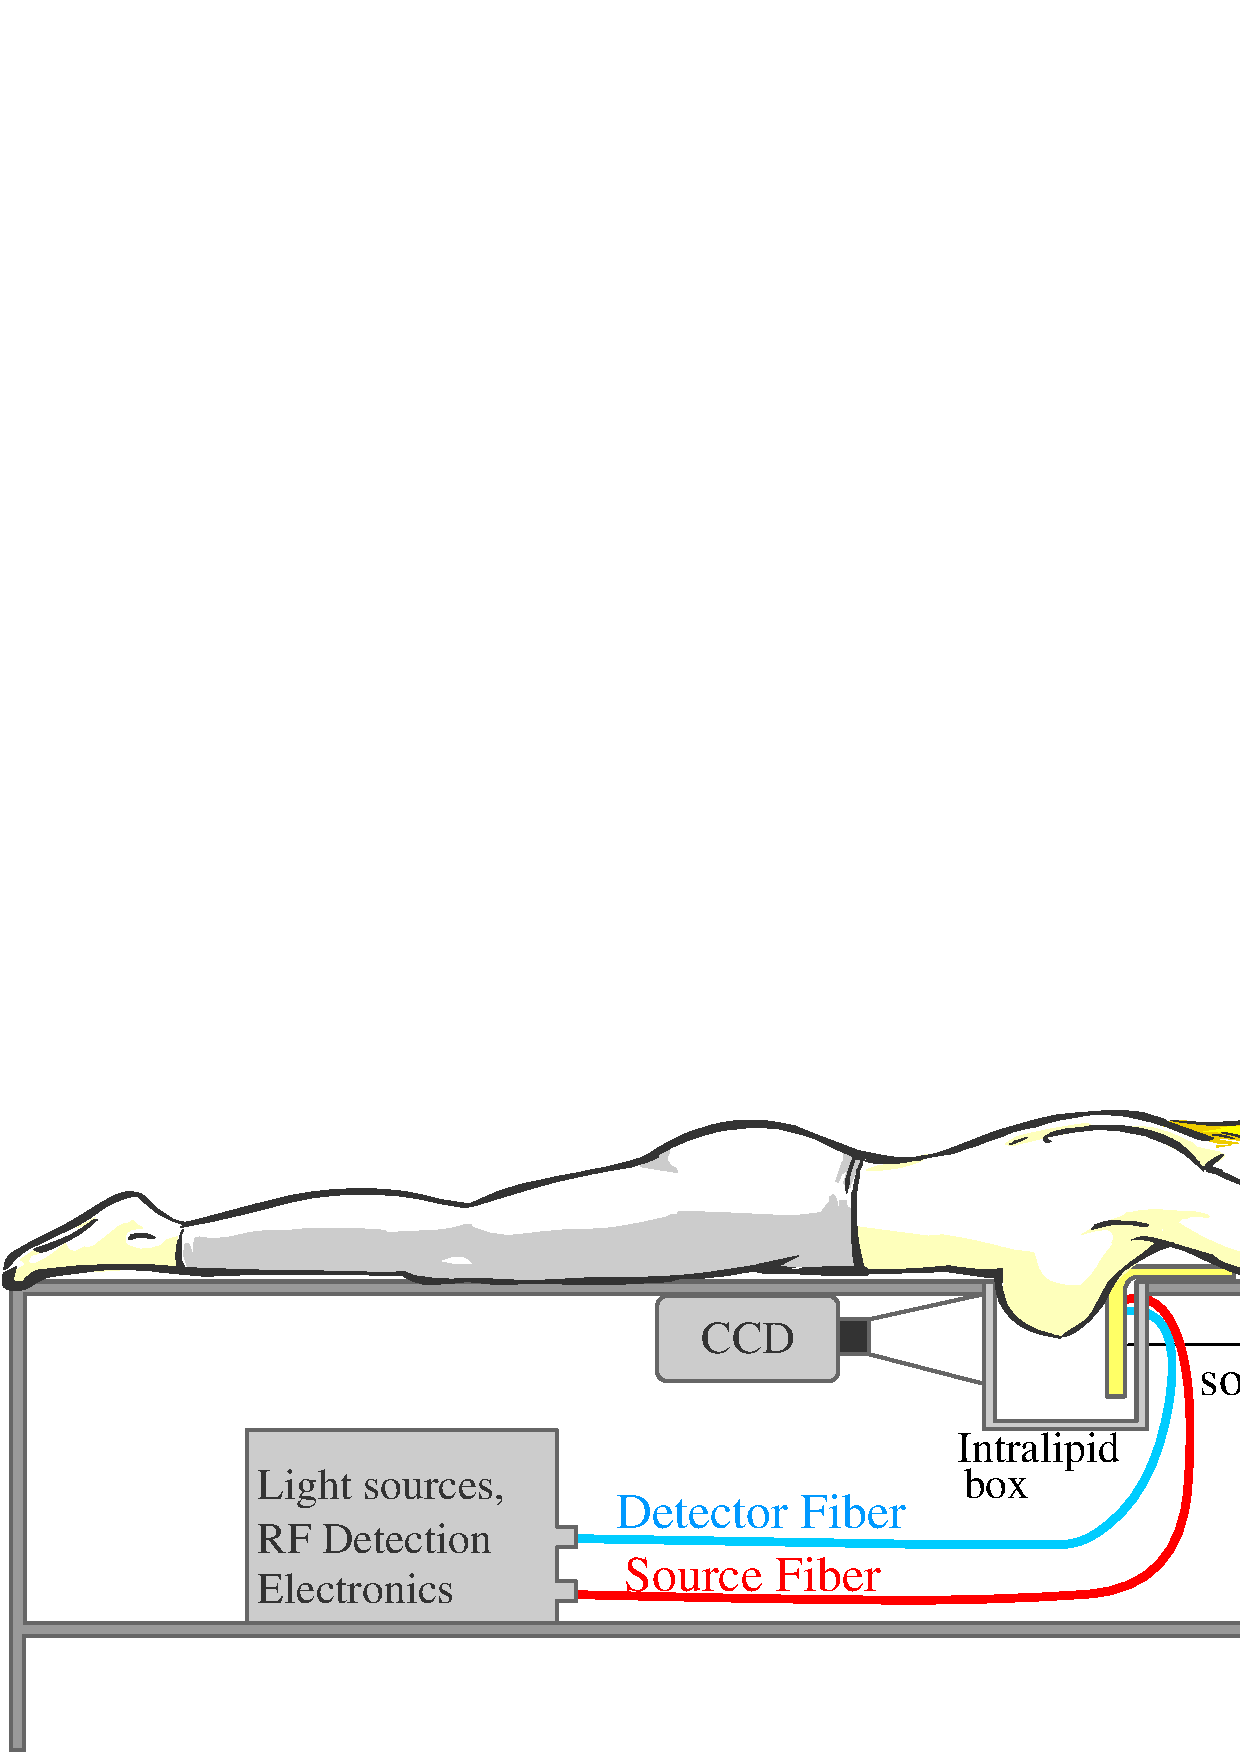
\includegraphics[width=14cm]{./figures/4_Gen3/gen2schem.png}
\caption{a) Picture of the previous generation breast scanner. b) CW and frequency-domain (FD)measurements are taken simultaneously. The patient lies prone and her breast is compressed axially with the sources and FD detectors on the top of the breast and the CCD detection window against the bottom of the breast. b) The source plate consist of 45 source position and 9 FD detectors with 16mm spacing between the sources. A subset of 984 detectors with $3\,{\rm mm}$ spacing is selected from the CCD for reconstruction.}
\label{fig:gen2schem}
\end{figure}
The Gen2 source plate has 45 fiber positions arranged in a 9x5 square grid with a spacing of 16 mm between nearest neighbors. The light is launched in series into the medium using cascading optical switches (DiCon Fiber Optics). At each source position, up to six different light source wavelengths were switched in (e.g., at wavelengths of 650, 690, 750, 785, 830, 905 nm) from the fiber-coupled diode lasers. On the detection side, a CCD camera (Roper Scientific, Trenton, NJ, VersArray:1300F) collected the exiting light in the transmission geometry. A full CCD image is obtained for each source (and laser combination) with an exposure time of ~500 ms. Thus, from each image a grid of data set is selected from the CCD after a $2\times 2$ hardware binning of the pixels. For the frequency-domain remission measurements, typically four lasers are modulated at $70\,{\rm MHz}$; measurements are made in remission with 3mm detector fibers arranged on the source plate in a $3\times3$ grid with $16\,{\rm mm}$ spacing. The light from these remission fibers are collected by an avalanche photodiode for homodyne frequency-domain analysis.

Of course, much was learned using this device, and these studies informed the design and development of my current DOT breast imager. Perhaps most significantly, it is difficult to eliminate the cross-talk between tissue absorption and scattering when employing only CW measurements (see Chapter 2), because both tissue parameters attenuate detected light when the intervening medium is turbid (e.g., like breast tissue). By using multispectral measurements and a few frequency-domain measurements in remission, we were able to ameliorate this problem to some degree. However, it was apparent that the apparatus would clearly benefit from a full frequency-domain approach as I aimed to do with my Gen3 instrument. Another problem concerned breast compression, which were carried out in the axial geometry; for comparison to other techniques such as MRI, the saggital compression geometry is better. Still another problem concerned instrumental drifts during the patient data-taking period which we did not take steps (in Gen2) to measure in-situ. In addition, we employed (in Gen2) only very crude means to define the breast boundaries in our early research; improvement in specification of the breast boundaries leads to direct improvements in our DOT image reconstructions. Finally, we wanted to improving the patient interface to increase patient comfort, breast coverage, and reduce the air-intralipid boundary that was present in the Gen2 instrument. Taken together, these potential improvements (as well as the potential for substantially more data with Gen3), drove us build a whole new instrument system.

\section{Clinical Breast Imaging Device (Gen3)}
The schematic for the Gen3 clinical breast imaging prototype that I built is shown in Fig.~\ref{fig:gen3schem}. Here, the patient lies prone and perpendicular to the modified biopsy bed while one breast is centered and sagittally compressed between the source plate and window in the breast tank. Typical thickness of compression varies between $56\,{\rm mm}$ and $70\,{\rm mm}$. As before, the tank is filled with a solution of intralipid and india ink mixture to match the optical properties of tissue of the patient in the NIR wavelength range.

The breast imager is composed of several key components. Briefly, the laser system encompasses optics and electronics for generating frequency-modulated light at various NIR wavelengths. This light sent through a custom switch to one of $209$ source positions on the inside a breast tank wherein the breast is inserted. The breast tank has two sets of profilometry cameras and projectors for determination of the breast boundary and 3D segmentation for the image reconstruction. Finally, gain-modulated detection is applied to the transmitted light using an image intensifer mounted on the CCD-camera apparatus. 
\begin{figure}[ht]
\centering
\includegraphics[width=14.5cm]{./figures/4_Gen3/gen3pic3.png}
\caption{Then breast imaging device in the mammography wing of Perelman Center for Advanced Medicine at the University of Pennsylvania (DONT HAVE RECENT PICTURES, WILL TAKE THIS WEEK SIMILAR TO OLD PICTURES WITH GOOD VIEW OF COMPONENTS)}
\label{fig:gen3pic}
\end{figure}
\begin{figure}[ht]
\centering
\includegraphics[width=14cm]{./figures/4_Gen3/gen3schem.png}
\caption{Schematic of the DOT breast imager. The system uses heterodyne detection which involves RF modulating the source and detection at slighly different frequencies. Five RF modulated laser modules are switch through in series for multi-spectral data. A $1\times 210$ galvo switch switches the light through 209 source positions and a calibration source on a source plate. The patient breast is inserted in the tank between the source plate and window. Profilometry devices on either side of the tank images the sides of the breast. Laser light exiting the tank window is measured by a RF gain-modulated image intensifier and CCD.}
\label{fig:gen3schem}
\end{figure}
First and foremost, my DOT breast imaging device improved on the Gen2 instrument through the incorporation of multispectral frequency-domain laser source illumination and a CCD-based heterodyne detection enabled by gain-modulation of an image intensifier placed between the sample output and the CCD-detector. This new capability dramatically improves separation of tissue absorption from tissue scattering and this improves the quantification capability of the 3D DOT reconstruction. Furthermore, by using an improved CCD camera for detection, we were able to collect a very large number ($10^6$) of source-detector pairs in parallel for improved resolution and image fidelity; in fact, my instrument collects the largest number of source-detector pairs compared to any DOT instrument in the world today. I will describe how these components work in later sub-sections of this chapter.

The temperature in hospital rooms might not be well controlled and the shift from CW to FD electronics make the instrument susceptible to additional problems that cause long term drifts and jitters in signal. These are especially true when working with RF electronics and long fibers ($\>5\,{\rm m}$). To address these issues we have have engineered not only front-end solutions like RF shielding and temperature controls to improve laser signal stability, but active concurrent reference measurements for real time signal correction and normalization. These improvements are further discussed in Sec.~\ref{sec:datanorm}.

As noted above, every 3D reconstruction benefits from knowledge of the breast boundary. In principle, one could use the slab boundary conditions and reconstruct the boundary directly, but in practice, if one knows where the boundary is, then one can segment the reconstruction and reduce the number of unknowns in the inverse probem. To this end, a pair of profilometry imaging systems were designed and built into the new instrument (discussed in Sec. \ref{sec:profilometry}) to provide 3D surface information about the breast shape. This required overcoming several engineering challenges such as capturing images in the same compression as the DOT data, building electronics with small space constraints (imaging within $<6cm$ spacings), compensating and calculating surface information where these images could not be acquired, and developing fast acquisition speeds in hardware and software.

Finally, significant effort was made to build a clinical grade device with a patient interface that maximized comfort and minimized movement during our measurement. To that end we designed the bed around a modified biopsy bed. The biopsy bed is also designed to get the maximum breast insertion underneath the bed from which we also benefit from as it gives us greater access to tumors that lie closer to the chest wall. In addition, much effort was put into the design of the software for the imager to enable simple and streamlined operation by our clinical collaborators with minimal training. These improvements are further detailed in Sec.~\ref{sec:clinicalui}.

\subsection{Breast Tank and Patient Bed}
The breast imaging system is built around a modified biopsy patient bed. The bed allows for more of the breast to be inserted into the tank for greater breast coverage. A translating head-rest was added to the bed to improve neck positioning and comfort. In addition we use an ultrasound bed for the patient to lie perpendicular to the biopsy bed. The breast tank is located right below the hole in the biopsy patient bed. The tank consists of a source plate made out of black delrin that is rail mounted to maintain parallel compression between the source plate and window. On the opposite side is an acrylic window with anti-reflective coating in the NIR. The space between the window and the detection setup is covered by a light box with a black felt inner lining prevents stray light and reflections from reaching the image intensifier and CCD. The tank is also mounted above a ball-bearing surface which allows the breast tank, light box, and detection system to rotate 90 degrees for either sagittal or axial compression of the breast. The frame underneath the bed was custom made with 80/20 aluminum T-slot frames that allow for customizability and easy modification in the future. The frame rolls on four castor lock wheels for easy movement and rigidity during measurements. Since the stainless steel bed is of considerable weight, hydrolic lifts were added to aid maintainence and experiment setup during non-clinical use.
\begin{figure}[ht]
\centering
\includegraphics[width=10cm]{./figures/4_Gen3/gen3bed.png}
\caption{ Picture of the a) biopsy bed and b) the translating head rest. c) Picture of the patient lying prone on the biopsy bed.}
\label{fig:gen3bed}
\end{figure}
\begin{figure}[ht]
\centering
\includegraphics[width=10cm]{./figures/4_Gen3/gen3tank.png}
\caption{Schematic of the gen3tank. Coordinates are those used in reconstruction and breast profilometry describe in Sec.~\ref{sec:profilometry}}
\label{fig:laserpic}
\end{figure}

\begin{figure}[ht]
\centering
\includegraphics[width=10cm]{./figures/4_Gen3/gen3hydrolics.png}
\caption{Hydrolic system installed on the Gen3 bed. Picture of the bed with a) hydrolics raised and b) lowered.}
\label{fig:hydrolics}
\end{figure}

\subsection{Laser System}
Source plate illumination is provided by a set of diode lasers operating the wavelengths of $660$, $690$, $785$, $808$, and $830\,{\rm nm}$, respectively. Table \ref{fig:lasertable} provides detailed characteristics of each laser module (Fig.~\ref{fig:laserpic}). (SAY WHAT LIGHT POWER COMES OUT OF LASERS TYPICALLY AND HOW THIS IS DECREASED (by what factor) AS IT TRAVERSES THE SYSTEM TO THE BREAST.) The diode lasers are mounted on a custom copper block inserted with a thermistor and a thermoelectric cooler (TEC) for temperature cooling and control at $-13^{\circ}{\rm C}$. Each laser diode is driven and temperature controlled by a dedicated ILX mainframe module (instrument info). The Gen2 instrument used controllers based around the simple driver (Thorlabs, IP500) and lacked temperature controls for its lasers. The CW stability of each laser is less than $0.5\%$ over a 3 hour periods. The lasers are amplitude modulated at $70\,{\rm MHz}$ using a an RF signal from a frequency generator (Rhode and Schwartz, SMB100). More specifically, the $70\,{\rm MHz}$ RF signal from the frequency generator is combined with the DC current from the ILX driver for each laser with a bias-tee (Mini-circuits, ZFBT-4R2G). The DC and RF voltage input for each laser was optimized using RF amplifiers (Mini-circuits, ZHL-2010+) and RF attenuators (Mini-circuits, VAT series). The laser driver current is optimized for the best modulation depth ($80\%$) and a sinusoidal waveform. The frequency modulated light from each fiber coupled laser is then coupled to a 6x1 100 $\mu m$ core optical switch (Optojenna) which allows the system to switch wavelengths in series.
\begin{figure}[h]
\centering
\includegraphics[width=10cm]{./figures/4_Gen3/RFlaser.png}
\caption{OLD PICTURE WILL REPLACE. Picture of the laser box. RF signal (from frequency generator outside of box) is split into five branches which are each sent through 20dBm amplifiers before being attentuated to appropriate voltages before being input into each laser box.}
\label{fig:RFlaser}
\end{figure}

%\begin{figure}[h]
%\centering
%\includegraphics[width=10cm]{./figures/4_Gen3/laserpic.png}
%\caption{a) picture and b) schematic of the laser module. There are three inputs to the laser module: 1) the RF modulation and the 2) DC current drive - which are combined by the bias-tee - as well as 3) the TEC voltage which drives the cooling element. There are two outputs: 1) the photodiode (if available) and the 2) thermistor. These outputs provide feedback for the current and temperature control respectively. The cold side of the TEC element cools the copper block to the desired temperature while the heat is dumped into the module case.}
%\label{fig:laserpic}
%\end{figure}


%\begin{figure}[h]
%\centering
%\includegraphics[width=10cm]{./figures/4_Gen3/laserbox.png}
%\caption{OLD PICTURE WILL REPLACE. Picture of the laser box. RF signal (from frequency generator outside of box) is split into five branches which are each sent through 20dBm amplifiers before being attentuated to appropriate voltages before being input into each laser box.}
%\label{fig:laserbox}
%\end{figure}

%\begin{table}[t]
%\centering
%\begin{tabular}{|c|c|c|c|c|c|c|}
%\hline
%$\lambda$ & Diode laser & Pin type & spec. current & current &AC input & power\\ 
%(nm) & part no. & (Thorlabs) & typ./max (mA) & ILX (mA) & (dBm) & (mW) \\ \hline
%660 & HL6545MG & H & 170 / 210 & 110 & 23 & 45 \\
%690 & V2561-2 & C & 768 / 800 & 425 & 20 & 96 \\
%785 & L785P090 & C & 120 / 160 & 93 & 22 & 67 \\
%808 & L808P200 & A & 230 / 300 & 180 & 20 & 80 \\
%830 & L830P150 & C & 200 / 250 & 123 & 19 & 78 \\ \hline 
%\end{tabular}
%\caption{Laser inventory and specs used in the Gen3 device. Current from the ILX driver provides the DC current while the AC modulation comes from the frequency generator. The average output power is measured at the end of the pigtail fiber from the laser. Losses up to the source plate is around $80\%$.}
%\end{table}

\subsection{Source Position Switch and Source Plate}
The output fiber from wavelength switch is connected in series to a $95/5$ fiber beam splitter with the $5\%$ going to the pickoff for signal normalization (which will be discussed in Sec. \ref{sec:datanorm}) and $95/5$ going to a custom 1x210 channel optical galvo-switch. Switching through 210 channels with a conventional cascade of switches used in the previous system based on mechanical or prism switch mechanisms is costly, slow, and have high throughput losses. For comparison, the Gen2 system switching speed between sources were $0.3$ to $0.5\,{\rm s}$ and had an average throughput of $50\%$. More importantly, the old switch had a heterogeneity of throughputs which ranged from $10\%$ to $80\%$ which resulted in a great variation in SNR between sources. The galvo switch has a more uniform throughput variation which resulted in differences in intensity no greater than $15\%$. In the galvo switch, input light from a $100\,\mu{\rm m}$ core fiber is collimated towards galvo-controlled mirrors which redirect light into a telecentric lens. The lens focuses the light onto a fiber bundle face with 210 $600\,\mu{\rm m}$ core fibers as shown in Fig \ref{fig:gen3switchschem}. The fiber from the bundle is connected to a a custom source fiber with $600\,\mu{\rm m}$ core. The source fibers were hand polished (to $98\%$ throughput) and fitted with FC/PC connector on the end towards the fiber bundle and a custom ferrule on the end which connects to the delrin source plate. The 209 source fibers are arranged on a 11x19 square grid on a black delrin plate with 8 mm spacing. The source plate is moved against the detection window and a picture is taken to determine source positions for reconstruction as shown in Fig.~\ref{fig:srcplatepic}. One of the remaining fibers is used as a calibration source and is thus placed far from the source grid. The purpose of this calibration source will be discussed in Sec.~\ref{sec:datanorm}. 
\begin{figure}[t]
\centering
\includegraphics[width=7cm]{./figures/Gen3switchschem.png}
\caption{Photograph of the (a) galvo switch and the (b) input face of the fiber bundle (c) custom patch cable (d) source plate
\label{fig:gen3switchschem}
\end{figure}
\begin{figure}[t]
\centering
\includegraphics[width=7cm]{./figures/Gen3switchpic.png}
\caption{Photograph of the (a) galvo switch and the (b) input face of the fiber bundle (c) custom patch cable (d) source plate
\label{fig:gen3switchpic}
\end{figure}

\begin{figure}[ht]
\begin{center}
\includegraphics[width=10.5cm]{./figures/4_Gen3/srcplatepic2.png}
\caption{Source plate picture taken by Breast Imager CCD after it has been moved up to the detection window. The fibers are backlit by illuminating the back of the fiber bundle. This picture is used to determine the source position for reconstructions.}
\label{fig:srcplatepic}
\end{center}
\end{figure}

%\begin{figure}[t]
%\centering\includegraphics[width=7cm]{./figures/BiopsyBedPic.png}
%\caption{\label{fig:BiopsyBedPic}
%  Photograph of the (a) galvo switch and the (b) input face of the fiber bundle
%\end{figure}

\subsection{Image Intensifier mounted CCD}
The detection system consists of a back-illuminated EMCCD (Andor iXon DV887, Ireland) with quantum efficiency optimized in the $500-700\,{\rm nm}$ range. One of the most attractive features of this CCD was its "frame transfer" function which allows for shutterless continous measurement which would be beneficial for our heterodyne measurement scheme in Sec. \ref{sec:heterodyne}. This CCD is mounted with a gain-modulated image intensifier (Lambert Instruments, II8MD GENIII, Netherlands) with a P43 Phosphor screen with a peak emission at $545\, {\rm nm}$. The lens element in front of the image intensifier is a Xenon $25\,{\rm mm}$ $f/0.95$ C-Mount Lens for 1-Inch CCD (Schneider Optics, Germany). The $512 \times 512$ pixel CCD is cropped to a field of view of the breast tank window with a $2 \times 2$ hardware binning for an image $155 \times 200$ pixels with a dpixel of $0.33\, {\rm mm/pixel}$ with a 16-bit depth. The gain on the image intensifier is modulated at  $70\,{\rm MHz} + 1 {\rm Hz}$

\subsection{Frequency-Domain Heterodyne detection}
\label{sec:heterodyne}
The primary goal of the DOT system is to measure the amplitude attenuation and phase shift of the input light as it transits through the breast tissue. There are two approaches to demodulate a high frequency RF signal to estimate $\delta A$ and $\delta phi$: homodyne and heterodyne. Homodyne systems have been developed for optical imaging \cite{Troy1996,Sevick-Muraca1997,Godavarty2003}, but here we describe the heterodyne approach.

Our system uses the well known optical heterodyne detection scheme [cite] where the input signal $\omega_{s}$ is nonlinearly mixed with a reference signal at the same frequency which is offset by a small cross correlation frequency $\omega_{cc}$ such that $\omega_{g}=\omega_{s}+\omega_{cc}$ and the resulting beat frequency at $\omega_{cc}$ is measured.  In our system, $\omega_{s}$ and  $\omega_{g}$ are produced by a pair of phase-locked frequency generators. The lasers in the devices are modulated at $\omega_{s}=70\,{\rm MHz}$ such that the light source intensity can be described as
\begin{equation}
I(t) = I_{0} + I_{\omega}\cos(\omega_s t+\phi_I)
\end{equation}
where  $I_{0}$ is the DC amplitude, $I_{\omega}$ the AC amplitude and $\phi_I$ is the phase offset of the laser. When the light passes through our breast tank diffusively through breast or intralipid solution the resulting transmitted light has the form
\begin{equation}
T(t) = I_{0}A_{DC}({\bf r}) + I_{\omega}A_{AC}\cos(\omega_s t +\phi_I+ \phi({\bf r}))
\end{equation}
where $A_0$, $A_{AC}$, and $\phi$ are the spatially varying DC, AC, and phase information that we are measuring from the surface of our diffusive breast or intralipid solution. On the detection side, we modulate the gain of the image intensifier at $\omega_{g}=70\,{\rm MHz} + 1 {\rm Hz}$ so that the image intensifier sensitivity is
\begin{equation}
G(t) = G_{0} +G_{\omega} \cos((\omega_s+\omega_{cc})t+\phi_G))
\end{equation}
\noindent
where $G_{0}$ is the DC amplitude, $G_{\omega}$ the AC amplitude and $\phi_G$ is the phase offset of the image intensifier gain. The signal that is detected by the CCD after the image intensifier is then
\begin{equation}
S = I(t) \times G(t) = (I_{0} + I_{\omega}\cos(\omega_s t+\phi_I))(G_{0} +G_{\omega}\cos((\omega_s+\omega_{cc})t+\phi_G)).
\label{4_signal}
\end{equation}
The CCD measures the light intensity out of the image intensifer at rate of $10\, {\rm frames/s}$ with frame transfer mode with an exposure time $\sim100\, {\rm ms}$ which in addition to the phosphor screen response time of the image intensifier of $\sim{\rm ms}$ acts as a low pass filter on the signal. Thus (Eqn \ref{4_signal}) simplifies to
\begin{equation}
\label{eqn:heterodyne}
S  = I_{0}G_{0}A_{DC}({\bf r}) + I_{\omega}G_{\omega}A_{AC}\cos(\omega_{cc}t+\phi_I-\phi_G+\phi({\bf r})).
\end{equation}
where we are able to measure $I_{0}G_{0}A_{DC},\,I_{\omega}G_{\omega}A_{AC}$ and $\phi_I-\phi_G+\phi$ for each CCD pixel.

\subsection{DOT measurement and timing}
The measurement timing is controlled using a National Instruments DAQ board (serial) which has an onboard clock as well as analog and digital I/O which can be programmed via Labview software on a computer. The DAQ board is programmed to put out two syncronized clocked TTL signals at $10\,{\rm MHz}$ and $0.5\,{\rm Hz}$. The $10\,{\rm MHz}$ goes to the reference input of the two frequency generators to phase lock the two together. The 0.5Hz signal is sent to the CCD to trigger the beginning of the 17 sequential measurement series synchronizing to the heterodyne measurement via the frequency generators.

In our measurement protocol we switch through all the source positions for each wavelength in series. The measurement at each source position is two seconds long (each triggered by the $0.5\,{\rm Hz}$ signal) resulting in a total measurement time per scan of $2\,{\rm s} \times 209\,{\rm sources} \times 5$ wavelengths $\sim 35$ minutes. For each two second measurement, 17 exposures are captured at at $10\,{\rm frames/s}$ for a total of $1.7\,s$. The remaining $300 {\rm ms}$ is used to write data from the camera buffer to the computer harddrive and switch to the next source position and/or wavelength. To get the $I_{0}G_{0}A_{DC},\,I_{\omega}G_{\omega}A_{AC}$ and $\phi_I-\phi_G+\phi$ from the heterodyne measurement mentioned in Sec. \ref{sec:heterodyne}, the time series (over 17 frames) light intensity for each pixel is fit to Eqn. \ref{eqn:heterodyne} fitted for these variables as shown in Fig. \ref{fig:timeseries}. 
\begin{figure}[ht]
\begin{center}
\includegraphics[width=14.5cm]{./figures/4_Gen3/timeseries.eps}
\caption{a) single time frame of light measured by the CCD. b) light intensities for pixels over time. This data is fit for DC, A, and $\phi$.}
\label{fig:timeseries}
\end{center}
\end{figure}

\section{Data Normalization}
\label{sec:datanorm}
A single breast scan will allow us to determine $I_{0}G_{0}A_{DC},\,I_{\omega}G_{\omega}A_{AC}$ and $\phi_I-\phi_G+\phi$ as we saw in Sec. \ref{sec:heterodyne}. However, the quantities that we are interested in are $A_{DC},\,A_{AC}$ and $\phi$ due to the optical properties of the breast. By taking a second reference scan with just the intralipid solution, we can divide out $I_{0}G_{0},\,I_{\omega}G_{\omega}$ and subtract out $\phi_I-\phi_G$.

In addition, we use a pickoff channel shown in Fig \ref{fig:gen3schem} to correct for any changes in amplitude or phase due to laser or RF instabilities before the galvo switch. 5 percent of the light is diverted using a 95/5 optical beam splitter and the fiber is run in front of the window with a 1-inch thick white delrin placed in front of the fiber tip used as a diffuser as shown in Fig \ref{fig:pickoffpic.jpg}. Because it is placed in the FOV of the window, this measurement is taken concurrently with each source measurement. An attenuator has been added to the pickoff so that the light level will be appropriate for the gain and dynamic range of the DOT measurement. 

Finally, we have one additional source of normalization that is used. The device has one additional source channel from the galvo switch which is placed very far from where the breast will be measured as shown in Fig \ref{fig:srcplatepic}. We call this the calibration source. Since it is just another source position fiber, this measurement is not taken concurrently, but rather in series with the DOT measurements. The calibration measurement is typically taken after every 10 sources. The advantage of this source is that is that unlike the pickoff, the calibration source corrects for the galvo and the reference tank and is useful for correcting long-term drifts in the system.

\section{Profilometry}
\label{sec:profilometry}
\subsection{Basics of Profilometry}
\begin{figure}[ht]
\begin{center}
\includegraphics[width=14.5cm]{./figures/4_Gen3/profcoord.png}
\caption{a) Profilometry setup which consist of a ccd camera and a portable projector. b)the schematic with the coordinate systems for the camera, projector, and the world or object coordinate.}
\label{fig:profcoord}
\end{center}
\end{figure}
To improve our reconstruction quality, we have built two sets of imaging devices based on fringe projection profilometry technique. A review on various implementation of this technique can be found in \cite{}. We chose to implement the techniques proposed by Zhang et. al \cite{Zhang2006} with an emphasis on speed, reduced dependance on a need for projector gamma calibrations (which are time consuming). 
Fig. \ref{fig:profcoord} shows the picture of the profilometry device and the corresponding schematic with the related coordinate systems for the camera, projector, and the world or object coordinate. The basic principle of fringe projection profilometry is to project fringe patterns onto an object and to map the phase shift of the patterns to the object height. To accomplish this, one must calibrate the profilometry device to determine the spatial transform function between the camera, projector, and object coordinates. Then a calibration to determine the one-to-one function between the phase shift and object height. The calibration methods for this is detailed in the following references \cite{Peng2007,Zhang2010,Gorthi2010,Geng2011}.

Once the calibrations are set, obtaining the 3D surface profile of an object (in our case the breast surface) requires three steps: 1) projecting fringe patterns onto the object and measure the fringe distortions (Eqn. \ref{eqn:fringe}, 2) convert the distorted images into a phase map, and 3) unwrapping the phase as the phase map is limited to [$-\pi, \pi$].
\noindent
{\bf Step 1:} Project fringe patterns with the following equations:
\begin{eqnarray}
\label{eqn:fringe}
I_{c,1}(x_c,y_c) & = & I_{c,dc}(x_c,y_c)+I_{c,ac}(x_c,y_c)\cos(\phi_c(x_c,y_c)-2\pi/3)\nonumber \\
I_{c,2}(x_c,y_c) & = & I_{c,dc}(x_c,y_c)+I_{c,ac}(x_c,y_c)\cos(\phi_c(x_c,y_c))\nonumber\\
I_{c,3}(x_c,y_c) & = & I_{c,dc}(x_c,y_c)+I_{c,ac}(x_c,y_c)\cos(\phi_c(x_c,y_c)+2\pi/3)
\end{eqnarray}
\noindent
where $I_{c,dc}$ is the average intensity, $I_{c,dc}$ is the modulation amplitude and $\phi_c$ is the phase value to be solved to extract our high information. The subscript $c$ denotes that this is in the camera reference.
\noindent
{\bf Step 2:} convert into phase map by solving for $\phi_c$ using Eqn. \ref{eqn:fringe} which gives us
\begin{equation}
\phi_c(x_c,y_c)=\arctan\big(\frac{\sqrt{3}(I_{c,1}(x_c,y_c)-I_{c,3}(x_c,y_c)}{2I_{c,2}(x_c,y_c)-I_{c,3}(x_c,y_c)}\big).
\end{equation}
\noindent
{\bf Step 3:} Unwrap $\phi_c$ to get the unwrapped phase
\begin{equation}
\Phi_c(x_c,y_c)= \phi_c(x_c,y_c)+2\pi\cdot k(x_c,y_c)
\end{equation}
where $k$ is found by projecting an additional set of images on the object to encode binary information in the image as proposed by Zhang et. al \cite{Zhang2006}. The schematic diagram of the projections used and the binary encoding method is shown in Fig \ref{fig:profunwrap}. Implementing these steps, we are able to unwrap the phase in the steps are shown in Fig \ref{fig:proffringe}.
\begin{figure}[ht]
\begin{center}
\includegraphics[width=14cm]{./figures/4_Gen3/profunwrap.png}
\caption{a) binary and fringe projections from the projector. b) unwrapping scheme proposed by Zhang et al. using the binary information encoded by the binary projections.}
\label{fig:profunwrap}
\end{center}
\end{figure}
\begin{figure}[ht]
\begin{center}
\includegraphics[width=14cm]{./figures/4_Gen3/proffringe.png}
\caption{a) object image b) fringe patterns projected onto object c) phase image d) unwrapped phase image.}
\label{fig:proffringe}
\end{center}
\end{figure}

\subsection{Profilometry for DOT segmentation}
The pair of profilometry devices we built are mounted on the DOT breast imager as show in Fig \ref{fig:proftank}. Fig \ref{fig:profdata} shows data from a human subject. Fringe pattern data is collected from each of the two profilometry devices as well as a sagittal image from the CCD where the outer edge has been traced by hand with a red line. The two surface point cloud generated by the profilometry phase map is combined with the outer trace (red line) of the breast image from the CCD to generate a 3D surface fit to generate a surface on the bottom side of the breast that was not illuminated by the profilometry projectors. This 3D surface fit is then used to generate a tetrahedral mesh to be used in the DOT image reconstruction.

\begin{figure}[ht]
\begin{center}
\includegraphics[width=12cm]{./figures/4_Gen3/proftank.png}
\caption{a) Front view of profilometry system with respect to Gen3 breast tank from perspective front CCD camera b) top view}
\label{fig:proftank}
\end{center}
\end{figure}
\begin{figure}[ht]
\begin{center}
\includegraphics[width=12cm]{./figures/4_Gen3/profdata.png}
\caption{ a) fringe pattern projected on the breast (left side of tank) b) fringe pattern on right side of tank c) sagittal view of breast from front CCD. Red line shows outer edge of breast traced by hand.}
\label{fig:profdata}
\end{center}
\end{figure}
\begin{figure}[ht]
\begin{center}
\includegraphics[width=14.5cm]{./figures/4_Gen3/proffit.png}
\caption{ a) 3D point cloud generated by fringe profilometry b)  surface fit of 3D point cloud c) line trace (red) from front CCD camera scaled and translated to match side surfaces d) 3D surface fit of whole breast generated from fringe profilometry data and front image trace.}
\label{fig:proffit}
\end{center}
\end{figure}

\section{Device characterization and testing}

\section{Clinical Results}